\section{Introduction}
\label{sec:intro}
%\KZ{The first two paras are too long and wordy. Get into the repeatition
%problem immediately please. I think if you can show some attention map or
%figures that illustrate why repeatition happens and what gives rise to our
%approach in the intro, this will be a strong motivation of our approach.}

Abstractive summarization is the task of creating a short, accurate,
informative and fluent summary from a longer text document.
It attempts to reproduce the semantics and topics of original text
by paraphrasing. 
Recently, sequence to sequence (seq2seq)
models~\cite{RushCW15,ChopraAR16,NallapatiZSGX16,SeeLM17,PaulusXS17}
have made great progress on abstractive summarization.
%Seq2seq model based on RNN and attention mechanism \cite{RushCW15} 
%was originally used for machine translation %\cite{SutskeverVL14,BahdanauCB14}.
%Gehring~\shortcite{gehring2017convs2s} proposed a convolutional 
%sequence to sequence model equipped with
%Gated Linear Units \cite{DauphinFAG17}, residual connections \cite{HeZRS16}
%and attention mechanism. 
%Based on CNN seq2seq model, Fan~\shortcite{FanGA18} presented a summarization model that
%can produce summaries that follow user preferences.
%Liu~\shortcite{LiuLZ18} extended the CNN seq2seq model by %controlling length
%of the summaries. The model has the ability to generate summaries in desired length
%in a natural manner. 
State-of-the-art solutions of the task are mainly based on 
convolutional (CNN seq2seq) models with attention 
mechanism~\cite{gehring2017convs2s,FanGA18,LiuLZ18}.
Convolutional networks are more effective for sequence modeling
and train much faster due to easier parallelism 
than recurrent networks~\cite{bai2018empirical}.
%network is a more powerful toolkit for sequence modeling than recurrent network.
%Convolutional model is much faster than the previous recurrent models as
%it can be easily parallelized.
Furthermore, unlike recurrent models, the convoluational models have
more stable gradients because of its backpropagation path. 
Thus, we take CNN seq2seq model as our basic model for the task.

However, just like the recurrent models, CNN-based models often produce
summaries with substantial repeated word sequences.
\tabref{tab:example} illustrates one such example by a
test case from the well known CNN/Daily Mail summarization dataset. 
In this case, the basic CNN produces two 
identical sentences (italized) in the result. 

\begin{table}[th]
\begin{center}
\scriptsize
%\begin{tabular}{lclclclclclclc}%{|p{7cm}|rl|}
\begin{tabular}{|l|}%{|p{7cm}|rl|}
\hline \bf Source document \\
\hline manchester city are rivalling manchester united and arsenal for valenciennes \\
       teenage defender dayot upamecano . the 16-year-old almost joined united in the \\
	   january transfer window only for him to opt to stay in france for a few more \\
	   months . centre-back umecano has played for france at u16 and u17 level. \\
	   monaco , inter milan and paris stgermain had also expressed interest . \\
	   \textbf{fourth-placed city face aston villa at the etihad stadium on saturday .} \\
\hline \bf Reference summary \\
\hline dayot upamecano was close to signing for manchester united in january . \\
       the 16-year-old, however , opted to stay in france with valenciennes . \\
	   centre-back upamecano has played for france at u16 and u17 level . arsenal are \\
	   also interested in the defender as man city join chase . \\
\hline \bf Basic CNN model (CNN) \\
\hline \textit{manchester city face aston villa at the etihad stadium 
on saturday .} the\\ 
	16-year-old almost joined united in the january transfer window . 
	   \textit{manchester}\\
	   \textit{city face aston villa at the etihad stadium on saturday .}\\
\hline
\end{tabular}
\end{center}
\caption{\label{tab:example} A test case from CNN/Daily mail 
and summary generated by the basic CNN model}
\end{table}



Unlike machine translation or paragraphing tasks in which the output words
and input words are almost one-to-one aligned, the output of summarization
is ``compressed'' from the input document. Naturally, every sentence or 
word sequence in the summary corresponds to one or more places in the source
document. If there were two identical word sequences in the summary,
they must be looking at and summarizing the same ``spots'' in the source.
This is evident from the attention map for the three sentences generated by 
CNN, shown in \figref{fig:attn_map}. The 1st and 3rd sentence attend to
the same location in the source (marked by the red boxes), while the second
sentence attends to another separate location in the source. The two
attention maps in the red boxes are very similar.

\begin{figure}[th!]
\centering
\subfigure[Attention distribution]{
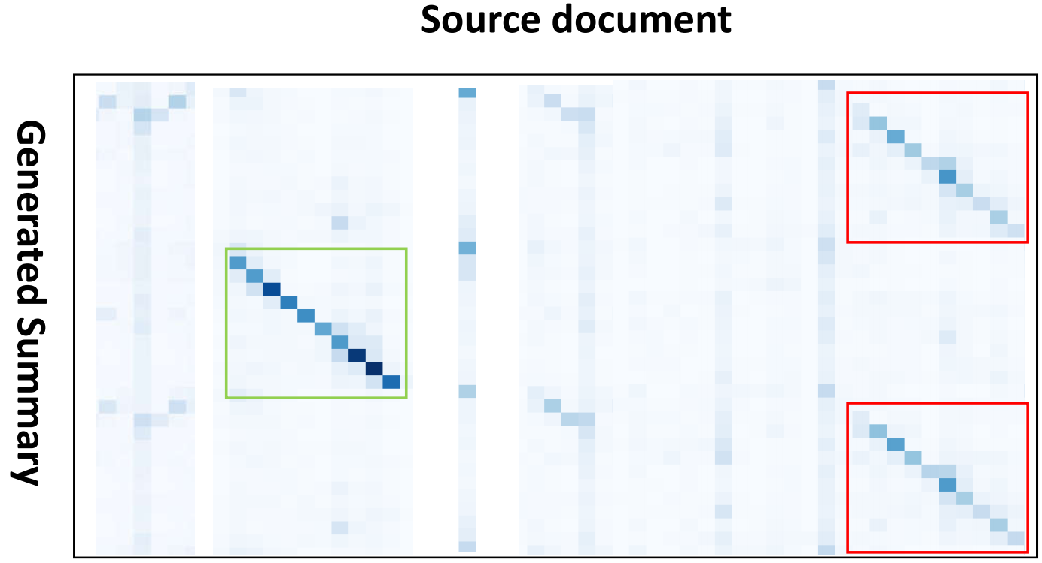
\includegraphics[width=0.8\linewidth]{map}
}
\quad
\subfigure[Green box]{
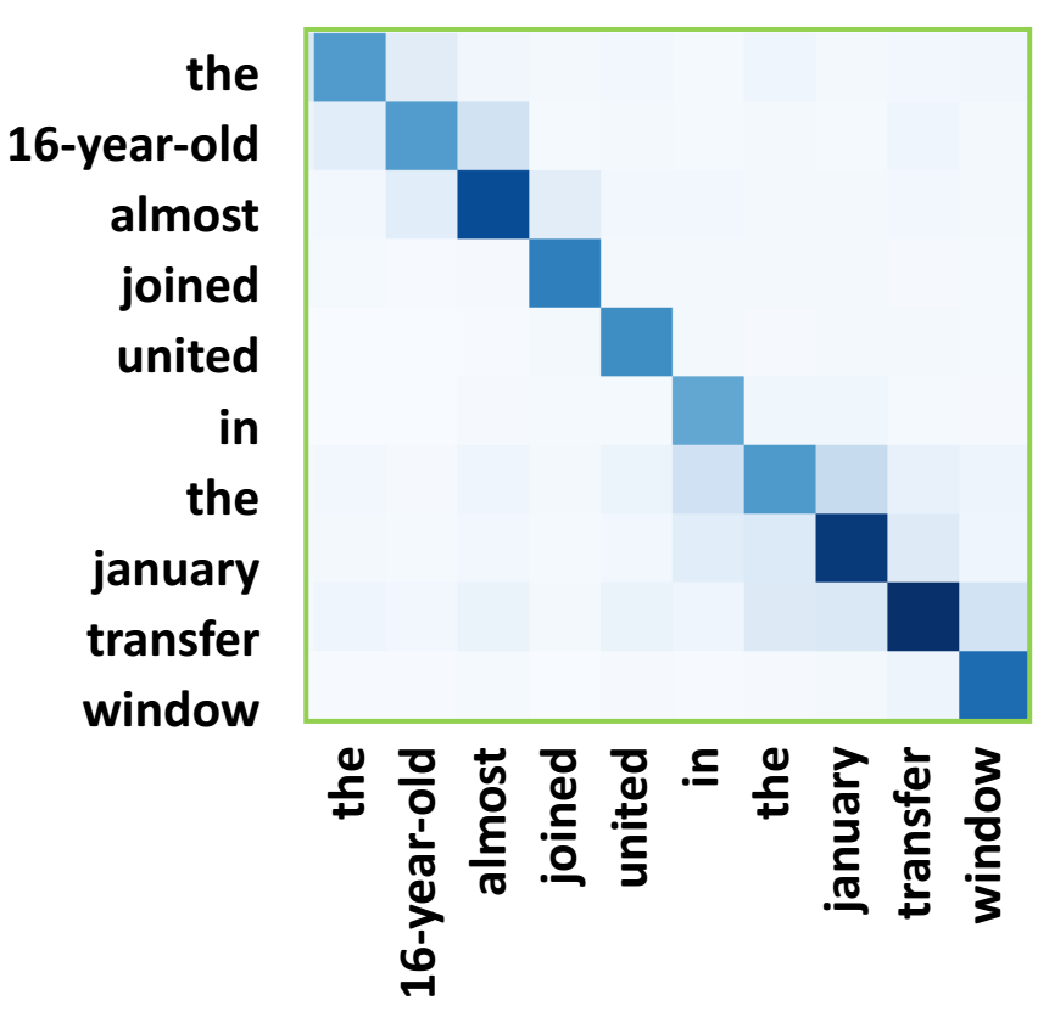
\includegraphics[width=0.4\linewidth]{map_1}
}
\quad
\subfigure[Red box]{
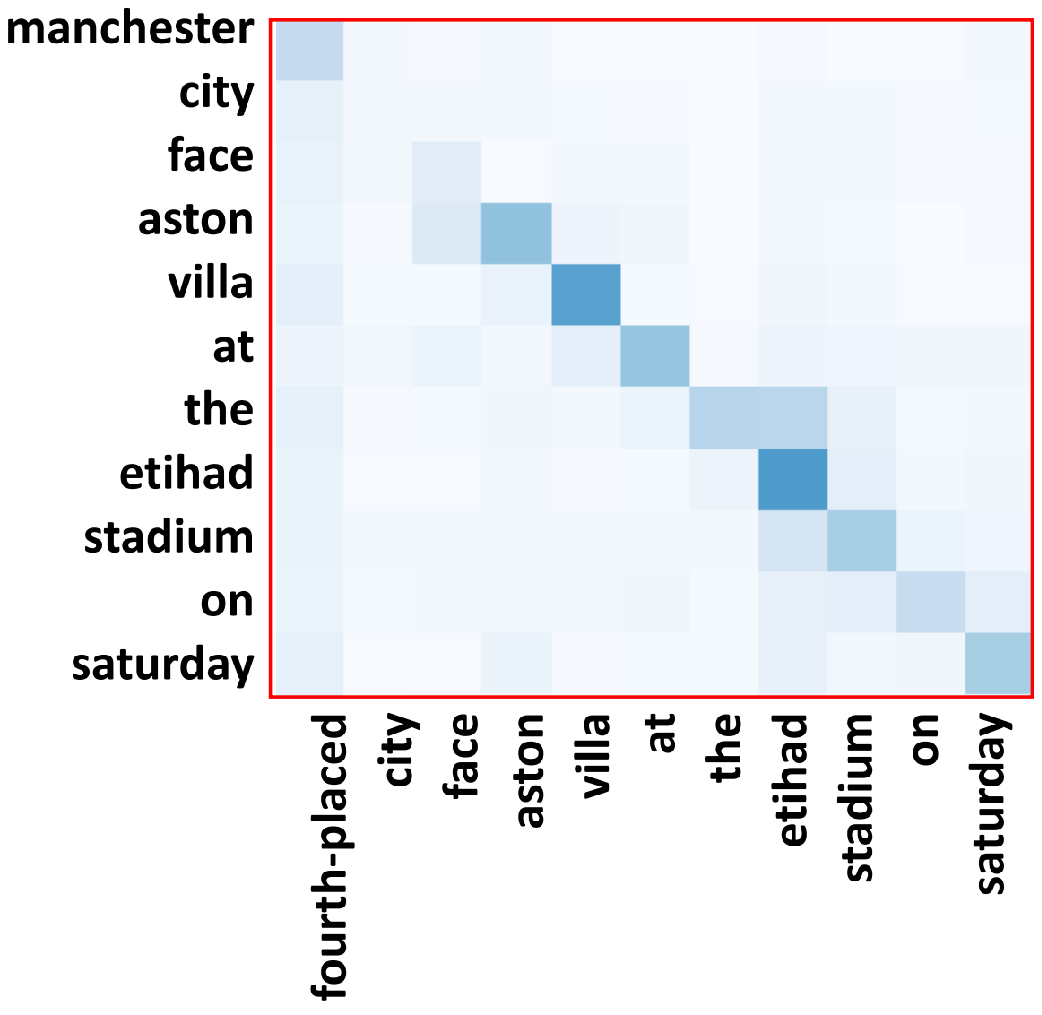
\includegraphics[width=0.4\linewidth]{map_2}
}
\caption{Attention distribution for example on basic CNN seq2seq model 
in \tabref{tab:example}}
\label{fig:attn_map}
\end{figure}


Driven by this intuition, a few efforts have been focusing on ``remembering''
what has been focused on before in the decoding process. 
For example, See~\shortcite{SeeLM17}  
uses coverage which is the sum of
attention distributions of all previously generated words to keep track of 
what has been summarized.  Paulus~\shortcite{PaulusXS17} and 
Fan~\shortcite{FanGA18} use intra-temporal 
attention\cite{NallapatiZSGX16} as well as intra-decoder attention to avoid 
attending to the same parts in the source document by 
revising attention scores while decoding. 
While these approaches discourage repetition to some extent,
they do so in an indirect manner, i.e., they do not 
make use of the attention information in source document directly.
Consequently, they may still generate repeated phrases, 
especially in long sentences (shown in \tabref{tab:strong_methods}).

\begin{table}[th]
\begin{center}
\scriptsize
%\begin{tabular}{lclclclclclclc}%{|p{7cm}|rl|}
\begin{tabular}{|l|}%{|p{7cm}|rl|}

\hline \bf Coverage model (COV) \\
\hline \textit{manchester city face aston villa at the etihad stadium on saturday .} 
       manchester \\
       city are rivalling manchester united and arsenal for valenciennes . 
	   \textit{ manchester} \\
	   \textit{city face aston villa at the etihad stadium on saturday .}\\
\hline \bf Intra-temporal attention (ITA) \\
\hline \textit{manchester city face aston villa at the etihad stadium on saturday .} 
	   \textit{ manchester} \\
	   \textit{city face aston villa at the etihad stadium on saturday .}\\
\hline \bf Intra-temporal $+$ Intra-decoder (ITDA) \\
\hline \textit{manchester city are rivalling manchester united and arsenal }for valenciennes \\
       teenage . manchester city face aston villa at the etihad stadium on saturday . \\
	   \textit{manchester city are rivalling manchester united and arsenal }. \\
\hline \bf Trigram decoder (TRI) \\
\hline \underline{defender dayot upamecano} has played for \underline{france} 
at unk and unk level .\\ 
       manchester city face aston villa at the etihad stadium on saturday . \\
%\hline \bf Backtracking decoder \\
%\hline the 16-year-old almost joined united in january transfer window . manchester \\
%       city face aston villa at the etihad stadium on saturday .\\ 
%\hline \bf Our(Attention Filter) \\
%\hline manchester city are rivalling manchester united and arsenal for defender dayot \\
%       upamecano . the 16-year-old joined in the january transfer window only for \\
%	   him to opt to stay in france . \\
\hline \bf Ours (Attention Filter + Backtracking decoder) \\
\hline manchester city face aston villa at the etihad stadium on saturday . the \\
       16-year-old almost joined united in the january transfer window . manchester \\
	   city are rivalling manchester united and arsenal for teenage defender daypot \\
	   upamecano .\\
\hline
\end{tabular}
\end{center}
\caption{\label{tab:strong_methods} Summaries generated by repetition
reducing methods }
\end{table}

\KZ{Notice I used the term ``POI'' below. You can use it throughout the paper.}
In this paper, we propose an attention filter mechanism that directly 
redistributes the attention from each word in the output summary to the source. 
It does so by computing the parts of interest (POIs) in the source document
per segment in the summary, and then minimizing the attention stores of
words in these POIs that have already been attended to in the preceding 
segments during decoding. 
Different segments in summary thus do not attend to the same spots
of source document, and hence there is no repetition. 
This is different from previous approaches
that they did not exactly pinpoint these parts in the source,
which we believe is critical in reducing the repetition. 
%\KZ{shall we back this up in experiment?}
%This kind of partial attention 
%can help us to pinpoint the corresponding location that each segment is
%attending to. Then we use attention filter to filter
%a partial attention from normal attention of each tokens in the other sections
%by minimizing the attention scores of attended location in source document.
%This can optimize the alignment relationship between source document and 
%summarization.  This is shown in \tabref{tab:attn_exp}. 

Despite the above effort, there are special cases, where similar sentences 
exist in the same source document, e.g.,

\fbox{
\parbox{0.9\columnwidth}{\small{``..the standout fixture in the league on saturday sees leaders 
	   chelsea welcome manchester united to stamford bridge , ... 
	   chelsea midfielder oriol romeu , 
\textbf{currently on loan at stuttgart} , predicts 
the scores for the weekend 's matches . romeu is \textbf{currently on a season-long 
loan at bundesliga side stuttgart .}''} 
}}

In this case, even if the decoder attends to different POIs of 
source document as it produces words, repetition may still result.  
One potential solution to this is a trigram decoder~\cite{PaulusXS17} 
which directly forbids the repeat of previously generated trigrams in
test time. While this simple but crude method avoids the repetition of any kind
completely, the meddling of the beam search at runtime causes another problem: 
it tends to generate sentences that are logically incorrect. 
In \tabref{tab:strong_methods} (TRI row), the defender dayot didn't
really play for France, according to the source document.
That is, the subject and object are mismatched.
So in this paper, we instead introduce a sentence-level backtracking decoder
that prohibits the repeat of the same sentence segment during testing time.
Our summary produced for the example is also shown in \tabref{tab:strong_methods}.

%In multiple-sentence summarization task, we observe that more often than not, repetition 
%occurs in the form of the same or similar sentences, rather than repetitive phrases 
%inside sentences. 
%On the other hand, it is prone to grammatical and factual errors(\tabref{tab:attn_exp}).
%Because it detects repetitive trigrams only by setting the 
%probability of the third word to zero. 
%It ignores that there are some same N-gram in the target summaries.
%The natural generation of a sentence is disturbed, giving rise to, 
%for example, mismatch of subject and object, and wrong phrases. 
%summarization is not a text generation problem which are are almost
%one-to-one correspondence between input and output words, it requires the model 
%has the ability to decide where to attend and where to ignore.
%The reason for repetition in abstractive summarization based on CNN seq2seq models is
%that the models always attend to the same location in the source document.
%As shown \tabref{tab:attn_exp} 
%and \figref{fig:attn_map} are corresponding. 
%Sentence in blue has factual erro. and \figref{fig:attn_map}.
%In the attention map, the darker color, the higher attention score.
%the repeated sentence in summary attends to the same location
%with high attention score, and different sentences attend to different location in source document. 
%

%Zhou~\shortcite{ZhouYWZ17} pointed out that there is no obvious alignment relationship 
%between the source text and the target summary, 
%and the encoder outputs contain noise for the attention. 
%Thus, removing repetition in abstractive summarization on CNN seq2seq model
%need a strong attention mechamism that can get alignment relationship
%between source document and target summary and determine the summarized
%parts in source documents directly. 

\cut{%%%%%%%%%%%%%%%%
as shown in \tabref{tab:src_rep}.
\figref{fig:attn_map3} shows that the repeated sentences
in summary respectively attend to the similar sentences in source document.
So we force our decoder to never output the same sentence more than once by a sentence level
backtraching decoder during testing. 

\begin{table}[th!]
\begin{center}
\scriptsize
\begin{tabular}{lclclclc}%{|p{7cm}|rl|}
\hline \bf Source document \\
\hline chelsea 's on loan midfielder oriol romeu goes up against sportsmail 's \\
       martin ... . the standout fixture in the league on saturday sees leaders \\
	   chelsea welcome manchester united to stamford bridge , ... \\
	   chelsea midfielder oriol romeu , \textbf{currently on loan at stuttgart} , predicts \\
	   the scores for the weekend 's matches . romeu is \textbf{currently on a season-long} \\
	   \textbf{loan at bundesliga side stuttgart .} \\
\hline \bf Reference summary \\
\hline oriol romeu is on a season-long loan at stuttgart from chelsea . the spanish \\
       midfielder predicts the scores in saturday 's matches . romeu goes \\
	   head-to-head with sportsmail 's martin keown . \\
\hline \bf Our(Attention Filter)\\
\hline chelsea beat manchester united on saturday . oriol romeu is currently \\
       on a season-long loan at stuttgart . oriol romeu is \\
	   currently on a season-long loan at the end of the season .\\
\hline \bf Our(Attention Filter + Backtracking decoder) \\
\hline chelsea face manchester united in the premier league on saturday . oriol romeu \\
       is currently on loan at stuttgart . \\
\hline
\end{tabular}
\end{center}
\caption{\label{tab:src_rep} Summaries generated by source document with repeatness. }
\end{table}


\begin{figure}[th!]
\centering
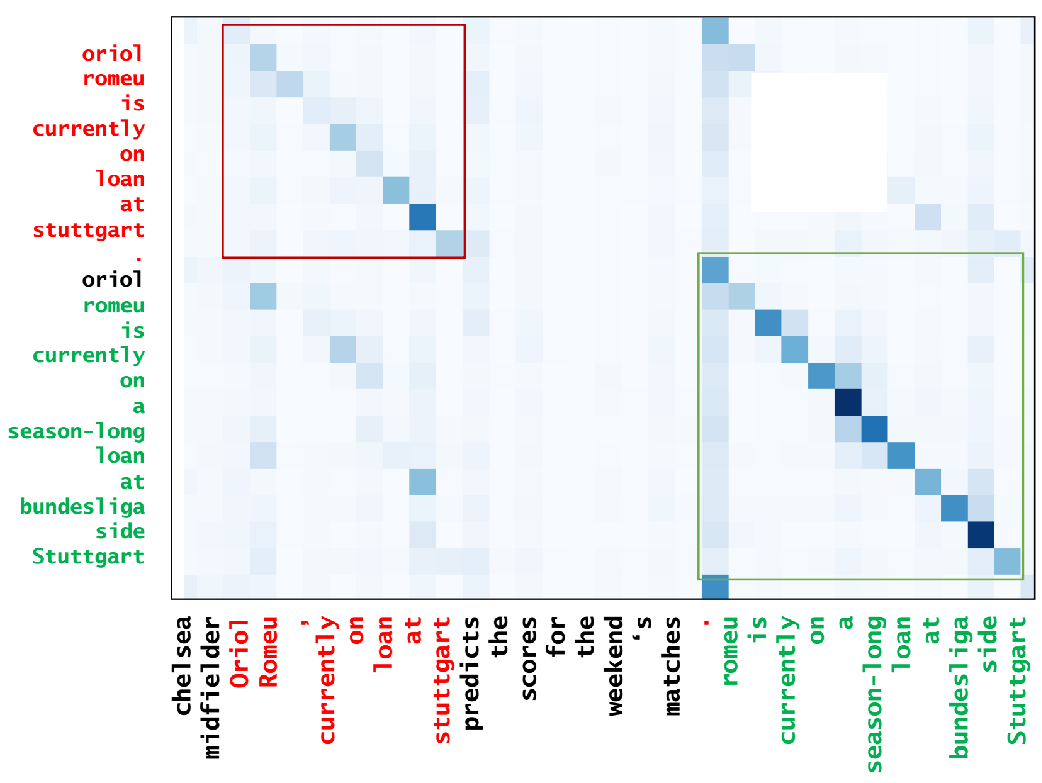
\includegraphics[width=0.9\linewidth]{map3}
\caption{Attention distribution(local) for our attention filter model in \tabref{tab:src_rep}}
\label{fig:attn_map3}
\end{figure}
}%%%%%%%%%%%%%%%%%%
%Compared with trigram decoder, we do not impact
%the process of beam search in the middle of a sentence, 
%which can reduce factual errors and grammatical erros(\tabref{tab:attn_exp}).

Our contributions are summarized as follows:
\begin{enumerate}
\item We identify the repetition problem in abstractive summaries generated
by CNN seq2seq models and propose new metrics to evaluate this problem.
\item We propose an effective approach that redistributes attention scores 
during training time, and guards against repetition by sentence backtracking
at runtime to reduce repetition in CNN seq2seq model (\secref{sec:approach}).
\item Our approach outperforms the state-of-the-art baseline methods 
substantially by all evaluation metrics, including accuracy, ROUGE scores, 
redundancy, repetition and correctness (\secref{sec:eval}).
\end{enumerate}

%Next, we present our approach based on convolutional sequence to sequence 
%model, followed by the evaluation of our approach and a discussion
%of related work. 
